%----------------------------------------------------------------------------------------
%	PACKAGES AND THEMES
%----------------------------------------------------------------------------------------
\documentclass[aspectratio=169,xcolor=dvipsnames]{beamer}
% \usetheme{SimplePlus}
\usetheme{metropolis}

\usepackage{hyperref,ragged2e}
\usepackage{graphicx} % Allows including images
\usepackage{booktabs} % Allows the use of \toprule, \midrule and \bottomrule in tables
\usepackage{physics,tensor,mathrsfs}
\usepackage{pgfgantt}
\usepackage{amsmath,amssymb,lmodern}
\usefonttheme{professionalfonts}
\geometry{paperwidth=145mm,paperheight=105mm}

% \setbeamertemplate{background} 
% {
%     \includegraphics[width=\paperwidth,height=\paperheight]{wallpaperflare.com_wallpaper 2.jpg}
% }


%----------------------------------------------------------------------------------------
%	TITLE PAGE
%----------------------------------------------------------------------------------------

\title[short title]{Gravitational instantons in Lovelock theory} % The short title appears at the bottom of every slide, the full title is only on the title page
\subtitle{In collaboration with: C.Corral, D.Flores and L. Sanhueza.}

\author[Pin-Yen] {Borja Diez B.}

\institute[NTU] % Your institution as it will appear on the bottom of every slide, may be shorthand to save space
{
    Instituto de Ciencias Exactas y Naturales \\
    Facultad de Ciencias\\
    Universidad Arturo Prat % Your institution for the title page
}
\date{19 de Enero de 2024} % Date, can be changed to a custom date


%----------------------------------------------------------------------------------------
%	PRESENTATION SLIDES
%----------------------------------------------------------------------------------------

\begin{document}

\begin{frame}
    % Print the title page as the first slide
    \titlepage
\end{frame}

\begin{frame}{Outline}
    \tableofcontents
\end{frame}

\section{Instantons}\justifying
\begin{frame}{Instantons in Yang-Mills theory}
The Yang-Mills action is given by
\begin{equation*}
    I_{\text{YM}}=\frac{1}{2 e^2}\int\dd^4x\sqrt{g}\Tr (F_{\mu\nu}F^{\mu\nu})
\end{equation*}
where
\begin{equation*}
    F_{\mu\nu}=\partial_\mu A_\nu-\partial_\nu A_\mu +[A_\mu,A_\nu].
\end{equation*}

The Yang-Mills equations of motion are
\begin{equation*}
    \nabla_\nu F^{\mu\nu}+[A_\nu,F^{\mu\nu}]=0 \quad \Leftrightarrow \quad D\star F=0
\end{equation*}
where $\star F$ is the dual of $F$,
\begin{equation*}
        \Tilde{F}_{\mu\nu}=\frac{1}{2}\epsilon_{\mu\nu\lambda\rho}F^{\lambda\rho}.
    \end{equation*}
\end{frame}

\begin{frame}{Instantons in Yang-Mills theory}\justifying
    The Chern-Pontryagin term is given by
    \begin{equation*}
        Q=\frac{1}{8\pi^2}\int\dd^4x\sqrt{g}\Tr\left(F_{\mu\nu}\Tilde{F}^{\mu\nu}\right).
    \end{equation*}
    The Yang-Mills action can be rewritten as
    \begin{align*}
        I_{\text{YM}}=\frac{1}{4e^2}\int\dd^4x\sqrt{g}\Tr \left(F_{\mu\nu}-\Tilde{F}_{\mu\nu}\right)^2+\frac{1}{2e^2}\int\dd^4x\sqrt{g}\Tr\left(F_{\mu\nu}\Tilde{F}^{\mu\nu}\right),
    \end{align*}
    so that
    \begin{equation*}
        I_{\text{{YM}}}-4\pi^2 Q=\frac{1}{4e^2}\int\dd^4x\sqrt{g}\Tr(F_{\mu\nu}-\Tilde{F}_{\mu\nu})^2\geq 0.
    \end{equation*}
    Self-dual configurations ($F_{\mu\nu}=\Tilde{F}_{\mu\nu}$), saturate this bound and are known as \textcolor{purple}{instantons}.\footnote{Belavin, Polyakov, Schwartz, Tyupkin, \textit{Phys. Lett. B} \textbf{59} (1975) 85.}
\end{frame}

\begin{frame}{Instantons in Yang-Mills theory}\justifying
\metroset{block=fill}
    \begin{block}{BPST instanton}
    \begin{equation*}
        A_\mu(x)=\frac{r^2}{r^2+\lambda^2}U^{-1}(x)\partial_\mu U(x)
    \end{equation*}
    where $\lambda$ is a constant and $U(x)\in SU(2)$.
    \end{block}
Let $\alpha\in \Omega^p(\mathcal{M})$, then
    \begin{equation*}
        \star\star \alpha = (-1)^{p(D-p)}\alpha. 
    \end{equation*}
    Evaluating self-dual configurations in the EOM's $D\star F=0$, we have
\begin{equation*}
    D\star\star F=\underbrace{DF\equiv 0}_{\text{Bianchi}}.
\end{equation*}
Thus, auto-dual configurations automatically satisfy the EOM's and  minimize the action for each homotopy class.
% Configuraciones auto-duales satisfacen automáticamente las ecuaciones de movimiento.
\end{frame}

\begin{frame}\justifying
$$\text{\textcolor{purple}{Will there be an analogue to these configurations in gravity?}}$$
\end{frame}

% \begin{frame}
% \begin{equation*}
%     \only<1>{I_{\text{YM}}=\qquad \int\dd ^4x\sqrt{g}\Tr(F_{\mu\nu}-\Tilde{F}_{\mu\nu})^2}
%     \only<2>{I_{\text{YM}}=\qquad \int\dd ^4x\sqrt{g}\underbrace{\Tr(F_{\mu\nu}-\Tilde{F}_{\mu\nu})^2}_{Tr(F_{\mu\nu})^2+\Tr(\Tilde{F}_{\mu\nu})^2-2\Tr(F_{\mu\nu}\Tilde{F}^{\mu\nu})}}
% \end{equation*}
% \end{frame}

% \begin{frame}
% $$\textcolor{violet}{I_{\text{YM}}=\frac{1}{2 e^2}\int\dd^4x\sqrt{g}\Tr (F_{\mu\nu}F^{\mu\nu})}$$\pause
% \begin{align*}
%         I_{\text{YM}}=\only<2>{&\textcolor{blue}{\#} \int\dd ^4x\sqrt{g}\Tr(F_{\mu\nu}-\Tilde{F}_{\mu\nu})^2}
% \only<3>{&\textcolor{blue}{\#} \int\dd^4x\sqrt{g}\left[\Tr(F_{\mu\nu})^2+\Tr(\Tilde{F}_{\mu\nu})^2-2\Tr(F_{\mu\nu}\Tilde{F}^{\mu\nu})\right]}
% \only<4>{&\textcolor{blue}{\#} \int\dd^4x\sqrt{g}\left[\Tr(F_{\mu\nu})^2+\textcolor{purple}{\underbrace{\Tr(\Tilde{F}_{\mu\nu})^2}_{\Tr(F_{\mu\nu})^2}}-2\Tr(F_{\mu\nu}\Tilde{F}^{\mu\nu})\right]}
% \only<5>
% {&\textcolor{blue}{\#} \int\dd^4x\sqrt{g}\left[2\Tr(F_{\mu\nu}F^{\mu\nu})-2\Tr(F_{\mu\nu}\Tilde{F}^{\mu\nu})\right]}
% \only<6>
% {&\textcolor{blue}{\frac{1}{4e^2}} \int\dd^4x\sqrt{g}\left[2\Tr(F_{\mu\nu}F^{\mu\nu})-2\Tr(F_{\mu\nu}\Tilde{F}^{\mu\nu})\right]}
% \only<7>
% {&\frac{1}{4e^2}\int\dd^4x\sqrt{g}\Tr(F_{\mu\nu}-\Tilde{F}_{\mu\nu})^2+\frac{1}{2e^2}\Tr(F_{\mu\nu}\Tilde{F}^{\mu\nu})}
% \only<8>
% {&\frac{1}{4e^2}\int\dd^4x\sqrt{g}\Tr(F_{\mu\nu}-\Tilde{F}_{\mu\nu})^2+\frac{1}{2e^2}\textcolor{purple}{\underbrace{\Tr(F_{\mu\nu}\Tilde{F}^{\mu\nu})}_{8\pi^2 C}}}
% \only<9>
% {&\frac{1}{4e^2}\int\dd^4x\sqrt{g}\Tr(F_{\mu\nu}-\Tilde{F}_{\mu\nu})^2+\frac{4\pi^2C}{e^2}}
% \end{align*}
% \end{frame}

% \begin{frame}
% $$\textcolor{violet}{I_{\text{YM}}=\frac{1}{2 e^2}\int\dd^4x\sqrt{g}\Tr (F_{\mu\nu}F^{\mu\nu})}$$
%     \begin{align*}
%         I_{\text{YM}}-\frac{4\pi^2 C}{e^2}=\only<1>{&\frac{1}{4e^2}\int\dd^4x\sqrt{g}\Tr(F_{\mu\nu}-\Tilde{F}_{\mu\nu})^2}
%         \only<2>
%         {&\textcolor{purple}{\underbrace{\frac{1}{4e^2}\int\dd^4x\sqrt{g}\Tr(F_{\mu\nu}-\Tilde{F}_{\mu\nu})^2}_{\geq 0}}}
%     \end{align*}
% \end{frame}

\begin{frame}{Gravitational instantons}\justifying
\metroset{block=fill}
\begin{block}{Gravitational instanton}\justifying
    Regular solutions of Einstein's field equations in the Euclidean in which curvature becomes zero at long distances.\footnote{Hawking, \textit{Phys. Lett. A} \textbf{60} (1977) 81.}
\end{block}
% \begin{itemize}
%     \item \textcolor{black}{Proporcionan una amplitud de tunelamiento entre estados de vacío topológicamente inequivalentes.}
%     \pause
%     \item La auto-dualidad se mide a nivel del \textcolor{red}{tensor de Weyl.}
% \end{itemize}
\end{frame}

\begin{frame}{Gravitational instantons}\justifying
    It defines $\Tilde{W}^{\mu\nu}_{\lambda\rho}$ as
    \begin{equation*}
        \Tilde{W}^{\mu\nu}_{\lambda\rho}=\frac{1}{2}\epsilon_{\mu\nu\alpha\beta}W^{\alpha\beta}_{\lambda\rho}.
    \end{equation*}
   The Chern-Pontryagin term in gravity is given by
    \begin{equation*}
        Q=\frac{1}{32\pi^2}\int\dd^4x\sqrt{|g|}\Tilde{R}^{\mu\nu}_{\lambda\rho}R^{\lambda\rho}_{\mu\nu}.
    \end{equation*}
Let us consider the Einstein-Hilbert action renormalized with the Gauss-Bonnet term
\begin{align*}
    I_{\rm EGB}
    % =\kappa\int\dd^4x\sqrt{|g|}\left(R+\frac{6}{l^2}+\frac{l^2}{4}\mathcal{G}\right)\\
    % 
    &=\frac{\kappa \ell^2}{16}\int\dd^4x\sqrt{|g|}\delta^{\mu_1...\mu_4}_{\nu_1...\nu_4}\left(R^{\nu_1\nu_2}_{\mu_1\mu_2}+\frac{1}{\ell^2}\delta^{\nu_1\nu_2}_{\mu_1\mu_2}\right)\left(R^{\nu_3\nu_4}_{\mu_3\mu_4}+\frac{1}{\ell^2}\delta^{\nu_3\nu_4}_{\mu_3\mu_4}\right),
\end{align*}
where $\kappa=(16\pi G_N)^{-1}$, $\Lambda\equiv-3/\ell^2$ and $\delta^{\mu_1\cdots\mu_k}_{\nu_1\cdots\nu_k}=k!\delta^{[\mu_1}_{[\nu_1}\cdots\delta^{\mu_k]}_{\nu_k]}$ is the generalized Kronecker delta. 

The EOM's associated with $I_{\rm EGB}$ are
\begin{equation*}
    R_{\mu\nu}+\frac{1}{2}Rg_{\mu\nu}+\Lambda g_{\mu\nu}=0\quad \Rightarrow \quad R_{\mu\nu}=-\frac{3}{\ell ^2}g_{\mu\nu}.
\end{equation*}
\end{frame}

\begin{frame}{Gravitational instantones}\justifying
    Einstein spaces satisfy
    \begin{equation*}
        W^{\mu\nu}_{\lambda\rho}=R^{\mu\nu}_{\lambda\rho}+\frac{1}{\ell^2}\delta^{\mu\nu}_{\lambda\rho}.
    \end{equation*}
    Evaluating $I_{\text{EGB}}$ in Einstein and self-dual spaces, we have \footnote{Miskovic \& Olea \textit{Phys. Rev. D} \textbf{79} (2009) 124024; Corral, Giribet \& Olea, \textit{Phys, Rev. D} \textbf{104} (2021) 064026.}
    \begin{align*}
        I_{\text{EGB}}&=\frac{\kappa \ell^2}{16}\int\dd^4x\sqrt{|g|}\delta^{\mu_1...\mu_4}_{\nu_1...\nu_4}W^{\nu_1\nu_2}_{\mu_1\mu_2}\tilde{W}^{\nu_3\nu_4}_{\mu_3\mu_4}\\
        &=\frac{\kappa \ell^2}{4}\int\dd^4x\sqrt{|g|}W^{\mu\nu}_{\lambda\rho}\tilde{W}^{\lambda\rho}_{\mu\nu}\\
        &=\frac{\kappa \ell^2}{4}\int\dd^4x\sqrt{|g|}R^{\mu\nu}_{\lambda\rho}\tilde{R}^{\lambda\rho}_{\mu\nu}\\
        &=8\pi^2\ell^2 Q.
    \end{align*}
\end{frame}

\begin{frame}{Lorentzian Taub-NUT-AdS metric}\justifying
The line element is given by \footnote{Taub, \textit{Annals Math.} \textbf{53} (1951) 472. Newman, Tamburino \& Unti \textit{J. Math. Phys.} \textbf{4} (1963) 915.}
\begin{equation*}
    \dd s^2=-f(r)(\dd t+2n\cos\theta\dd\phi)^2+\frac{\dd r^2}{f(r)}+(r^2+n^2)\dd\Omega^2_2
\end{equation*}
with
\begin{equation*}
    f(r)=\frac{r^2-n^2}{r^2+n^2}-\frac{2MGr}{r^2+n^2}+\frac{r^4+6n^2r^2-3n^4}{\ell^2(r^2+n^2)}.
\end{equation*}
\begin{itemize}
    \item It does not have curvature singularities.
    \item It has topological defects which contribute to gravitational entropy.\footnote{Hawking \& Hunter \textit{Phys. Rev. D} \textbf{59} (1999) 044025; Mann \textit{Phys. Rev. D} \textbf{60} 104047 (1999).}
\end{itemize}
\end{frame}

\begin{frame}\justifying
One can move the position of the string to by making an improper coordinate change of the form $t\to \tilde{t}=t+2n\phi C$, to make the position of the string unobservable.\footnote{Misner, \textit{J. Math. Phys.} \textbf{4} (1963) 924.}
\begin{figure}
    \centering
    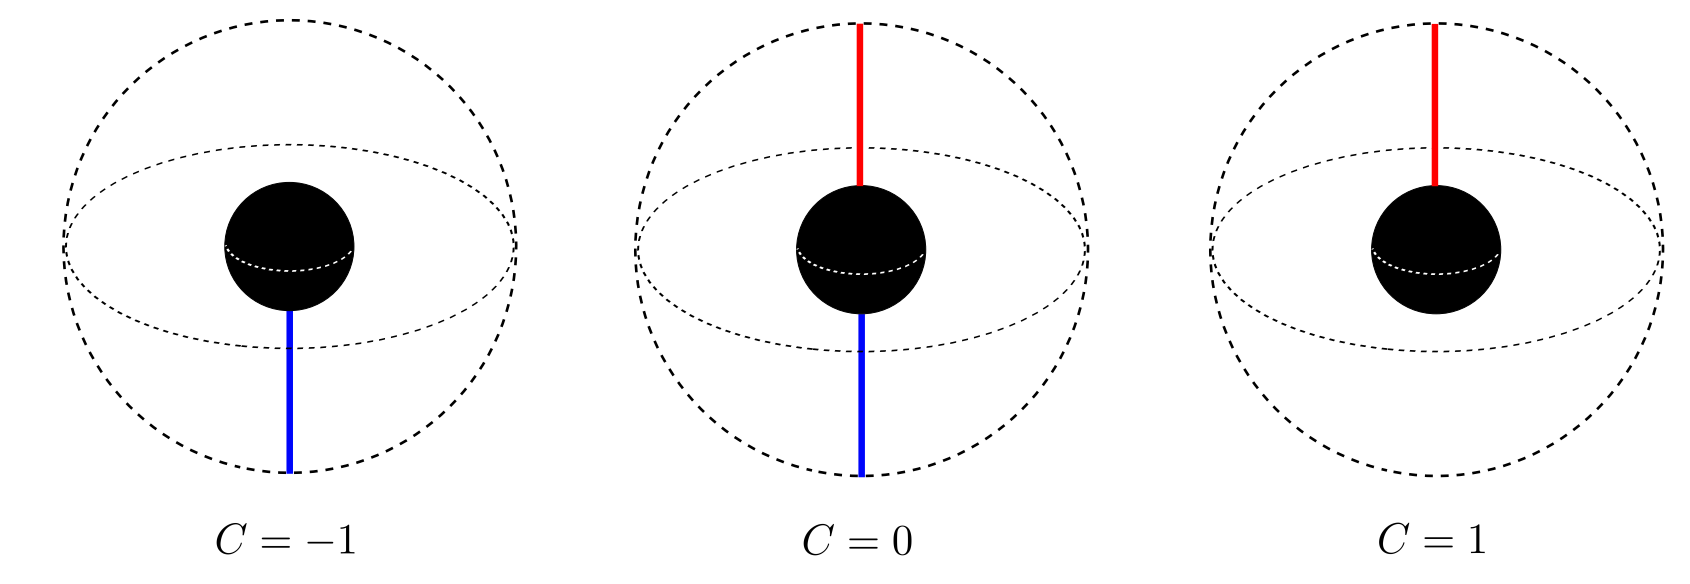
\includegraphics[scale=0.40]{Captura de pantalla 2024-01-08 a la(s) 14.33.59.png}
    \caption{Durka \textit{Int J. Mod. Phy. D} \textbf{31} (2023) 2250021.}
\end{figure}
\end{frame}


\begin{frame}{Euclidean Taub-NUT-AdS metric}\justifying
Through a double Wick rotation $t\to -i\tau$ and $n\to -in$ we obtain the Euclidean version of Taub-NUT,
\begin{equation*}
    \dd s^2=f(r)(\dd \tau+2n\cos\theta\dd\phi)^2+\frac{\dd r^2}{f(r)}+(r^2-n^2)\dd\Omega^2_2
\end{equation*}
with
\begin{equation*}
    f(r)=\frac{r^2+n^2}{r^2-n^2}-\frac{2MGr}{r^2-n^2}+\frac{r^4-6n^2r^2+3n^4}{\ell^2(r^2-n^2)}.
\end{equation*}
% Se puede imponer la condición de nut, resultando,
% \begin{equation*}
%     f_{\text{NUT}}(r)=\frac{r-n}{r+n}+\frac{(r-n)^2(3n+r)}{\ell^2(r+n)}
% \end{equation*}
We can choose between two conditions to require regularity,
\begin{align*}
    &\rm NUT:&f(n)=0&\qquad \rm y&\eval{f'(r)}_{r=n}=\frac{4\pi}{\beta_{\rm nut}}\\
    &\rm Bolt:&f(r_b)=0&\qquad \rm y&\eval{f'(r)}_{r=rb}=\frac{4\pi}{\beta_{\rm bolt}}
\end{align*}
% Para eliminar singularidades cónicas, se debe imponer un período de $8\pi n$ a la coordenada $\tau$.
\end{frame}


\begin{frame}{Maurier-Cartan forms of $SU(2)$}\justifying
    \begin{align*}
        \sigma_1&=\cos\psi\dd\theta + \sin\theta\sin\psi\dd\phi\\
        \sigma_2&=-\sin\psi\dd\theta+\sin\theta\cos\psi\dd\phi\\
        \sigma_3&=\dd\psi + \cos\theta\dd\phi
    \end{align*}
where
\begin{equation*}
    0\leq \theta\leq \pi,\quad 0\leq\phi<2\pi,\quad 0\leq\psi<4\pi
\end{equation*}
and satisfy the following relation
\begin{equation*}
    \dd\sigma_i+\frac{1}{2}\epsilon_{ijk}\sigma^j\wedge \sigma^k=0.
\end{equation*}
% El elemento de línea de la 2-esfera unitaria se puede escribir como
% \begin{equation*}
%     \dd\Omega^2_2=\sigma_1^2+\sigma_2^2
% \end{equation*}
Setting $\psi=\frac{\tau}{2n}$ we can write the Euclidean Taub-NUT metric in terms of the Maurier-Cartan forms
    \begin{align*}
        \dd s^2
        % &=f(r)4n^2(\dd\psi+\cos\theta\dd\phi)^2+\frac{\dd r^2}{f(r)}+(r^2-n^2)\dd\Omega_2^2\\
        &=f(r)4n^2\sigma_3^2+\frac{\dd r^2}{f(r)}+(r^2-n^2)(\sigma_1^2+\sigma_2^2).
    \end{align*} 
\end{frame}

% \begin{frame}{Métrica de Taub-Nut}\justifying
%     Haciendo $\psi=\frac{\tau}{2n}$ podemos escribir la métrica de Taub-NUT Euclídea en términos de las formas de Maurier-Cartan
%     \begin{align*}
%         \dd s^2&=f(r)4n^2(\dd\psi+\cos\theta\dd\phi)^2+\frac{\dd r^2}{f(r)}+(r^2-n^2)\dd\Omega_2^2\\
%         &=f(r)4n^2\sigma_3^2+\frac{\dd r^2}{f(r)}+(r^2-n^2)(\sigma_1^2+\sigma_2^2)
%     \end{align*}
% \end{frame}

\begin{frame}{Eguchi-Hanson metric}\justifying
Their line element is given by \footnote{Eguchi \& Hanson, \textit{Phys. Lett. B} \textbf{74}, 249 (1978); Eguchi \& Hanson \textit{Annals Phys.} \textbf{120}, 82 (1979); Calabi, \textit{Annales Scientifiques de l'École Normale Supérieure} \textbf{12}, 269 (1979).}
\begin{equation*}
    \dd s^2=\frac{r^2}{4}f(r)\sigma_3^2+\frac{\dd r^2}{f(r)}+\frac{r^2}{4}(\sigma_1^2+\sigma_2^2)
\end{equation*}
with
\begin{equation*}
    f(r)=1-\frac{a^4}{r^4}-\frac{\Lambda r^2}{6}.
\end{equation*}
\begin{itemize}
    \item When $\Lambda = 0$ is self-dual. ($W^{\mu\nu}_{\lambda\rho}=\tilde{W}^{\mu\nu}_{\lambda\rho}$).
    \item It has a bolt.
    \item Its hypersurfaces of constant $r$ are topologically $S^3/\mathbb{Z}_2$.
\end{itemize}
\end{frame}

\begin{frame}\justifying
    \begin{equation*}
        \text{\textcolor{purple}{What happens if we go to dimensions larger than $D=4$?}}
    \end{equation*}
\end{frame}



\section{Lovelock theory of gravity}

% \begin{frame}{Teoría de Lovelock}
% \textcolor{purple}{La generalización natural de la Relatividad General es la teoría de Lovelock.}
% \end{frame}
\begin{frame}{Lovelock theory}\justifying
Its action principle is given by \footnote{Lovelock, \textit{J. Math. Phys.} \textbf{12}, 498 (1971); Lanczos, \textit{Annals Math.} \textbf{39}, 842 (1938).}
    \begin{equation*}
        I[g_{\mu\nu}]=\sum_{p=0}^{\left[\frac{D-1}{2}\right]}\int_{\mathcal{M}}\dd^Dx\sqrt{|g|}\alpha_p\mathcal{L}^{(p)}
    \end{equation*}
with
\begin{equation*}
         \mathcal{L}^{(p)}=\frac{1}{2^p}\delta^{\mu_1\cdots\mu_{2p}}_{\nu_1\cdots\nu_{2p}}R^{\nu_1\nu_2}_{\mu_1\mu_2}\cdots R^{\nu_{2p-1}\nu_{2p}}_{\mu_{2p-1}\mu_{2p}}
\end{equation*}
where the associated equations of motion are
\begin{equation*}
    E^\mu_\nu=-\sum_{p=0}^{\left[\frac{D-1}{2}\right]}\frac{\alpha_p}{2^{p+1}}\delta^{\mu\mu_1\cdots\mu_{2p}}_{\nu\nu_1\cdots\nu_{2p}}R^{\nu_1\nu_2}_{\mu_1\mu_2}\cdots R^{\nu_{2p-1}\nu_{2p}}_{\mu_{2p-1}\mu_{2p}}.
\end{equation*}
\end{frame}

\begin{frame}\justifying
Properties:
 \begin{itemize}
        \item The action is built purely from the metric.
        \item It is invariant under general coordinate transformations (diffeomorphisms).
        \item It is invariant under local Lorentz transformations.
        \item It delivers equations of motion that are at most second order in derivatives of the metric.
        \item Torsion free.
        \item It propagates the same local degrees of freedom as General Relativity.\footnote{Henneaux, Teitelboim \& Zanelli \textit{Nucl. Phys. B} \textbf{332} (1990) 169.}
    \end{itemize}
\end{frame}




\section{Gravitational instantons in higher dimensions}\justifying
\begin{frame}{K\"ahler manifolds}
A manifold is K\"ahler if it is a manifold \textcolor{purple}{Riemaniann, complex and simplectic}, with these three structures compatible with each other.

\metroset{block=fill}
\begin{block}{Riemaniann manifold}
    $\mathcal{M}$ is a Riemaniann variety if it admits a non-degenerate metric whose \textcolor{blue}{eigenvalues} are all \textcolor{blue}{positive definite.}
\end{block}
\metroset{block=fill}
    \begin{block}{Complex manifold}
    $\mathcal{M}$ is a complex manifold of dimension $D$ if we can find complex coordinates with \textcolor{blue}{holomorphic transition functions} on a real $2D$-dimensional manifold.
    \end{block}
\end{frame}

\begin{frame}{K\"ahler manifolds}\justifying
\metroset{block=fill}
    \begin{block}{Simplectic manifold}
        Let's consider a Hermitian metric $\mathcal{M}$,
        \begin{equation*}
            \dd s^2=g_{a\bar{b}}\dd z^{a}\dd\Bar{z}^{\Bar{b}}.
        \end{equation*}
        The real 2-form of K\"ahler is defined as
        \begin{equation*}
            \Omega=\frac{i}{2}g_{a\bar{b}}\dd z^{a}\wedge \dd\bar{z}^{\bar{b}}=\bar{\Omega}.
        \end{equation*}
        A metric is said to admit a symplectic structure if \textcolor{blue}{$\dd\Omega=0$}.
By Poincaré's lemma, we can write locally
\begin{equation*}
    \Omega=\dd \mathcal{B}
\end{equation*}
where $\mathcal{B}=\mathcal{B}_\mu\dd x^\mu$ is the 1-form \textcolor{red}{K\"ahler potential.}
    \end{block}
\end{frame}

\begin{frame}\justifying
\metroset{block=fill}
\begin{block}{Generalization to higher dimensions.}
    Let us consider a family of metrics constructed from a $U(1)$ bundle of an Einstein-K\"ahler base-manifold of the form\footnote{Page \& Pope \textit{Class. Quant. Grav} \textbf{4} (1987) 213.}
    \begin{equation*}
        \textcolor{purple}{\dd s^2=h(r)f(r)(\dd\tau+\mathcal{B})^2+\frac{\dd r^2}{f(r)}+N(r)\dd\Sigma^2_{(D-2)}.}
    \end{equation*}
\end{block}
    \begin{itemize}
    \item If $h(r)=N(r)=\frac{r^2}{4}$ the Eguchi-Hanson metric is recovered.
    \item If $h(r)=4n^2$ and $N(r)=(r^2-n^2)$ the Taub-NUT metric is recovered.
\end{itemize}
\end{frame}

\begin{frame}{Wheeler polynomials}\justifying
\begin{itemize}
    \item Let us remember that the equations of motion in Lovelock's theory are at most second order in derivatives of the metric.
    % \item Al tomar el ansatz métrico anterior, ocurre que siempre la $E^\tau_\tau$ ($=E^r_r$) es de \textcolor{purple}{primer orden} para la función métrica $f(r)$.
    \item By taking a static ansatz of the form
    \begin{equation*}
        \dd s^2=-f(r)\dd t^2+\frac{\dd r^2}{f(r)}+r^2\dd\Sigma^2_{(k)}
    \end{equation*}
    It turns out that it is always possible to make a first integral over $E^t_t = (E^r_r)$, so that
    \begin{equation*}
    \sum_{n=0}^{\left[\frac{D-1}{2}\right]}H_n(r)f^n(r)+\mu = 0
\end{equation*}
where $\mu$ is a integration constant.\footnote{J. T. Wheeler \textit{Nucl. Phys. B} \textbf{273} (1986) 732.}
\end{itemize}
% \end{equation*}
\end{frame}

\begin{frame}
    $$\text{\textcolor{purple}{Will it be possible to do something similar but with a stationary ansatz?}}$$
\end{frame}
% \begin{equation*}
%     E^t_t(\#)=\dv{r}\left(\sum_{n=0}^{\left[\frac{D-1}{2}\right]}H_n(r)f^n(r)\right)=0
% \end{equation*}
% Esto nos permite hacer una primera integral \footnote{J. T. Wheeler \textit{Nucl. Phys. B} \textbf{273} (1986) 732.}
% \begin{equation*}
%     \sum_{n=0}^{\left[\frac{D-1}{2}\right]}H_n(r)f^n(r)+\mu = 0


\begin{frame}{Wheeler polynomials}\justifying
    In the literature, generalizations of Taub-NUT and Eguchi-Hanson have been studied in theories with corrections in higher order of curvature:   \begin{itemize}
    \item Charged Taub-NUT in Einstein-Gauss-Bonnet gravity.\footnote{Dehghani \& Mann \textit{Phys. Rev. D} \textbf{72} (2005) 124006.}
    \item Taub-NUT on $D=8$ at cubic order in the Lovelock series.\footnote{Hendi \& Dehghani \textit{Phys. Lett. B} \textbf{666},116 (2008).}
        \item Eguchi-Hanson in higher dimensions in $f(R)$ gravity.\footnote{Hendi, Mann, Riazi \& Eslam Panah \textit{Phys. Rev. D} \textbf{86}, 104034 (2012).}
        \item Taub-NUT/Bolt in higher dimensions in cubic gravity.\footnote{Bueno, Cano, Hennigar \& Mann \textit{JHEP} \textbf{10}, 096 (2018).}
        \item \textcolor{purple}{Taub-NUT in $D=8$ coupled with Maxwell fields at cubic order in the Lovelock series.}\footnote{Corral, Flores-Alfonso \& Quevedo \textit{Phys. Rev. D} \textbf{100} (2019) 064051.}
        \item \textcolor{purple}{Eguchi-Hanson in $D=8$ to cubic order in the Lovelock series.}\footnote{Corral, Flores-Alfonso, Giribet \& Oliva \textit{Phys. Rev. D} \textbf{106} (2022).}
    \end{itemize}
    % \begin{itemize}
    %     \item Corral, Flores-Alfonso \& Quevedo \textit{Phys. Rev. D} \textbf{100} (2019) 064051.
    %     \item Corral, Flores-Alfonso, Giribet \& Oliva \textit{Phys. Rev. D} \textbf{106} (2022) 084055.
    % \end{itemize}
\end{frame}

\begin{frame}\justifying
\begin{center}
    \textcolor{purple}{Will it be possible to find a polynomial of this type to order $n$ in Lovelock theory and in arbitrary dimension?}
\end{center}
\end{frame}


% \begin{frame}{Polinomios de Wheeler}
% \begin{itemize}
%     \item Recordemos que las ecuaciones de movimiento en la teoría de Lovelock son a lo más de segundo orden en derivadas de la métrica.
%     \pause
%     \item Al tomar el ansatz métrico anterior, ocurre que siempre la $E^t_t$ ($=E^r_r$) es de \textcolor{purple}{primer orden} para la función métrica $f(r)$.
% \end{itemize}
% \pause
% \begin{align*}
%     E^t_t=\dv{t}\left(\sum_{n=0}^{\left[\frac{D-1}{2}\right]}H_n(r)f^n(r)\right)
% \end{align*}


\section{Some novel results}
\begin{frame}{Local properties}\justifying
Choosing an orthonormal frame
    \begin{equation*}
    e^0=\frac{\dd r}{\sqrt{f(r)}},\qquad e^1=\sqrt{f(r)h(r)}(\dd\tau+\mathcal{B}),\qquad e^{i}=\sqrt{N(r)}\bar{e}^{i}
\end{equation*}
The components of the spin connection are given by
\begin{align*}
    \omega^{01}&=-\frac{(fh)'}{2h\sqrt{f}}e^1,\qquad 
    \omega^{0i}=-\frac{\sqrt{f}N'}{2N}e^{i}\\
    \omega^{1i}&=\frac{\sqrt{fh}}{2N}\Omega^{i}{}_je^j,\qquad 
    \omega^{ij}=\bar{\omega}^{ij}-\frac{\sqrt{fh}}{2N}\Omega^{ij}e^1\
\end{align*}
where $\dd \mathcal{B}\equiv \Omega=\frac{1}{2}\Omega_{ij}\bar{e}^{i}\wedge \bar{e}^j$. 
\end{frame}

\begin{frame}{Local properties}\justifying
The components of the Lorentz curvature are given by
    \begin{align*}
    R^{01}&=-\frac{1}{2\sqrt{h}}\left[\frac{(fh)'}{\sqrt{h}}\right]'e^0\wedge e^1-\frac{1}{2}\frac{N}{\sqrt{h}}\left[\frac{fh}{N}\right]'\Omega.\\
    R^{0i}&=-\frac{1}{2}\sqrt{\frac{f}{N}}\left[\frac{\sqrt{f}N'}{\sqrt{N}}\right]'e^0\wedge e^{i}-\frac{1}{4\sqrt{h}}\left[\frac{fh}{N}\right]'\Omega^{i}_{\ j}e^1\wedge e^j.\\
    R^{1i}&=\frac{1}{4\sqrt{h}}\left[\frac{fh}{N}\right]'\Omega^{i}_{\ j}e^0\wedge e^j+\frac{1}{2N}\sqrt{\frac{fh}{N}}\bar{D}_k\Omega^{i}_{\ j}e^k\wedge e^j \\
    &+\frac{1}{4N}\left[\frac{fh}{N}\Omega_k^{\ i}\Omega^k_{\ j}-\frac{N'(fh)'}{h}\delta^i_j\right]e^1\wedge e^j.\\
    R^{ij}&=\bar{R}^{ij}+\frac{1}{2N}\sqrt{\frac{fh}{N}}\bar{D}_k\Omega^{ij}e^1\wedge e^k-\frac{1}{2\sqrt{h}}\left[\frac{fh}{N}\right]'\Omega^{ij}e^0\wedge e^1-\frac{fN'^2}{4N^2}e^{i}\wedge e^j\\
    &-\frac{fh}{4N^2}\left(\Omega^{ij}\Omega_{kl}+\Omega^{i}_{\ k}\Omega^j_{\ l}\right)e^k\wedge e^l.
\end{align*}
\end{frame}
\begin{frame}{Eguchi-Hanson}\justifying
Considering different topologies for the Einstein-K\"ahler base manifold, i.e.,
    \begin{table}
    \centering
    \begin{tabular}{cccccc}
         &$\mathbb{CP}^k$  &$\mathbb{CH}^k$  & $(\mathbb{T}^2)^k$ & $(\mathbb{S}^2)^k$ & $(\mathbb{H}^2)^k$\\\hline
         $\gamma$& $1$ & $-1$ & $0$ &$1$  & $-1$\\\hline
         $\sigma$& $0$ & $0$ &$0$  &$1$  & $1$\\\hline
    \end{tabular}
    \caption{Dependence of the parameters on the topology of the base manifold.}
    \label{tab:2}
\end{table}
we find that the Wheeler polynomial at $D=2m$ for the generalization of the \textbf{Eguchi-Hanson} metric to order $n$ in the Lovelock series is
    \begin{equation*}
   a^{2m} +\sum_{l=0}^{n}\frac{\alpha_l(-4)^{l-1}m!(m-2)!}{(m-l-1)!(m-l+1)!}F_l(r)r^{2(m-l+1)}=0
\end{equation*}
where $a$ is a integration constant and
\begin{equation*}
     F_l(r)=\left(f(r)-\frac{2\gamma}{m}\right)^l+\sigma \sum_{k=0}^l(-1)^k\binom{l}{k}f(r)^{l-k}\left(\frac{2\gamma}{m}\right)^k\left(\frac{m^k(m-k)!}{m!}-1\right)
\end{equation*}
\end{frame}

\begin{frame}
We also consider an extension to electrovacuum by introducing $U(1)$ gauge fields, in which we consider the Lovelock-Maxwell theory in $D=2m$ dimensions, described by the action principle
\begin{equation}
  I[g_{\mu\nu},A_\mu] = \sum_{p=0}^{\left[\frac{D-1}{2} \right]}\int_{\mathcal{M}}\dd^D x \sqrt{|g|}\,\alpha_p\,{\mathscr{L}}^{(p)} - \frac{1}{4}\int_{\mathcal{M}}\dd^Dx\sqrt{|g|}\,F_{\mu\nu}F^{\mu\nu}
\end{equation}
where 
\begin{equation*}
  F_{\mu\nu }=\partial_\mu  A_\nu  -\partial_\nu  A_\mu 
\end{equation*}
is the $U(1)$ field strength. The field equations for the metric and the gauge potential are given by 
\begin{equation}
  E_{\mu\nu }=T_{\mu\nu },\qquad \nabla_\mu F^{\mu\nu }=0
\end{equation}
respectively, where $T_{\mu\nu }$ is the Maxwell's stress-energy tensor given by
\begin{equation}
  T_{\mu\nu }=F_{\mu\lambda}F_\nu ^{\lambda}-\frac{1}{4}g_{\mu\nu }F_{\lambda\rho }F^{\lambda\rho }
\end{equation}


\end{frame}

\begin{frame}{Charged Eguchi-Hanson}
	In order to solve this system, we consider an ansatz for the metric constructed out of the $U(1)$ fibration over Einstein-K\"ahler manifolds considered above together with a Maxwell field aligned along the direction of the fiber,
	\begin{equation*}
  A=A_\mu\dd x^\mu =a(r)(\dd t+\mathcal{B})
\end{equation*}
where the $\mathcal{B}$ is the K\"ahler potential $1$-form associated to the Einstein-K\"ahler base-manifold.

The Maxwell equations are solved by the following gauge potential profile
\begin{equation*}
  a(r)=\frac{q}{r^{2(m-1)}}+pr^2
\end{equation*}
where $q$ and $p$ are integration constants.
\end{frame}

\begin{frame}{Charged Eguchi-Hanson}
	Replacing the latter into the field equations for the metric, we find that the solution can be written in a generalized Wheeler's polynomial form given by
	\begin{equation*}
  0 = a^{2m} +\sum_{l=0}^{n}\frac{\alpha_l(-4)^{l-1}m!(m-2)!}{(m-l-1)!(m-l+1)!}F_l(r)r^{2(m-l+1)} + P(r)
\end{equation*}
where the contribution of the Maxwell fields $P(r)$ is
\begin{equation*}
  P(r) = \frac{4(m-2)}{m-1}\left(\frac{q^2}{r^{2(m-1)}}+\frac{r^{2(m+1)}}{m+1}p^2\right)+16pq r^2
\end{equation*}
\end{frame}

\begin{frame}{$\mathbb{CP}^2$ instanton generalization}
$\mathbb{CP}^2$ is a two dimensional complex manifold which may also be given a Fubini-Study metric. The fact that it has non-vanishing Pontrjagin number has led Eguchi and Freund to consider ir as an analogue of the $SU(2)$ Yang-Mills instanton.

Its generalization to higher dimensions can be obtained recursively, given rise to the $\mathbb{CP}^k$ spaces. We can even consider spaces with negative Gaussian curvature ($\mathbb{CH}^k$), in a similar way. 

A property of the $\mathbb{CP}^k$ and $\mathbb{CH}^k$ spaces is that they are Lovelock constants, that is, each tensor of the equations of motion is proportional to the metric. In this way, they are solutions of the Lovelock equations in $D=2k$ dimensions up to a polynomial constraint on the Lovelock couplings $\alpha_p$, given by
\begin{equation}
  \sum_{p=0}^k\frac{\alpha_p}{(k-p-1)!(k-p+1)!}\left(\frac{2\gamma}{k+1}\right)^{p-1}=0
\end{equation}
where $\gamma=1$ for $\mathbb{CP}^k$ and $\gamma=-1$ for $\mathbb{CH}^k$.

	
\end{frame}


%    We also consider the charged case using a Maxwell ansatz aligned to the direction of the $U(1)$ bundle. Solving the Lovelock-Maxwell equations,
%    \begin{align*}
%        E_{\mu\nu}&=T_{\mu\nu}\\
%        \nabla_\mu F^{\mu\nu}&=0
%    \end{align*}
%    where
%    \begin{equation*}
%        T_{\mu\nu}=F_{\mu\lambda}F_\nu^{\ \lambda}-\frac{1}{4}g_{\mu\nu}F_{\lambda\rho}F^{\lambda\rho}
%    \end{equation*}
%    we find that the vector potential takes the form
%    \begin{equation*}
%    A=A_\mu\dd x^\mu=\left(\frac{q}{r^{2(m-1)}}+p r^2\right)(\dd t+\mathcal{B})
%\end{equation*}
%and the Wheeler polynomial is
%\begin{align*}
%   &a^{2m} +\sum_{l=0}^{n}\frac{\alpha_l(-4)^{l-1}m!(m-2)!}{(m-l-1)!(m-l+1)!}F_l(r)r^{2(m-l+1)}\\&+\frac{4(m-2)}{m-1}\left(\frac{q^2}{r^{2(m-1)}}+\frac{r^{2(m+1)}}{m+1}p^2\right)+16pq r^2=0
%\end{align*}


% \begin{frame}{Resultados}
%     \begin{equation*}
%    a^{2m} +\sum_{l=0}^{n}\frac{\alpha_l(-4)^{l-1}m!(m-2)!}{(m-l-1)!(m-l+1)!}F_l(r)r^{2(m-l+1)}=0
% \end{equation*}
% con
% \begin{equation*}
%     F_l(r)=\sum_{k=0}^l(-1)^k\binom{l}{k}f(r)^{l-k}\left(\frac{2\gamma}{m}\right)^k\left(\frac{m^k(m-k)!}{m!}\right)^\sigma
% \end{equation*}
%     \begin{table}
%     \centering
%     \begin{tabular}{cccccc}
%          &$\mathbb{CP}^k$  &$\mathbb{CH}^k$  & $(\mathbb{T}^2)^k$ & $(\mathbb{S}^2)^k$ & $(\mathbb{H}^2)^k$\\\hline
%          $\gamma$& $1$ & $-1$ & $0$ &$1$  & $-1$\\\hline
%          $\sigma$& $0$ & $0$ &$0$  &$1$  & $1$\\\hline
%     \end{tabular}
%     \caption{Dependencia de los parámetros con la topología del base manifold.}
%     \label{tab:2}
% \end{table}
% \end{frame}

% \section{Planificación}
% \begin{frame}{Planificación}\justifying
%     \begin{enumerate}
%         \item Encontrar el polinomio de Wheeler para el caso con parámetro de nut.
%         \item Estudiar la estructura de nuts y bolts para métricas con parámetro de NUT.
%         \item Estudiar las propiedades globales de la solución.
%         \item Estudiar la termodinámica y las transiciones de fase.
%         \item Escribir la tesis.
%         \item Defensa de tesis.
%     \end{enumerate}
% \end{frame}


% \begin{frame}{Planificación}\justifying
%     \begin{figure}[h]
% \scalebox{0.85}{
% \begin{ganttchart}[vgrid,hgrid]{1}{18}
% \gantttitle{2024}{12}
% \gantttitle{2025}{6}\\
% \gantttitlelist{1,...,12}{1}
% \gantttitlelist{1,...,6}{1}\\
% \ganttbar{Objetivo 1}{1}{4}\\
% \ganttbar{Objetivo 2}{5}{7}\\
% \ganttbar{Objetivo 3}{3}{6}\\
% \ganttbar{Objetivo 4}{6}{9}\\
% \ganttbar{Objetivo 5}{8}{12}\\
% \ganttbar{Objetivo 6}{13}{15}
% \end{ganttchart}
% }
% \end{figure}
% \end{frame}

%------------------------------------------------

\begin{frame}
    \Huge{\centerline{\textbf{Thanks!}}}
\end{frame}

%----------------------------------------------------------------------------------------

\end{document}